\documentclass[10pt]{beamer}
\usepackage{amsmath}
\usepackage{amsthm}
\usepackage{tikz}
\usepackage{booktabs}
\usetikzlibrary{shapes.geometric,arrows}
\usepackage{listings}


%\usepackage{minted}


\newcommand{\R}{\mathbb{R}}
\newcommand{\C}{\mathcal{C}}
\renewcommand{\u}{\mathbf{u}}
\renewcommand{\v}{\mathbf{v}}
\newcommand{\w}{\mathbf{w}}
\newcommand{\x}{\mathbf{x}}
\newcommand{\y}{\mathbf{y}}
\renewcommand{\b}{\mathbf{b}}
\newcommand{\e}{\mathbf{e}}
\newcommand{\s}{\mathbf{s}}


\newcommand{\A}{\mathbf{A}}
\newcommand{\B}{\mathbf{B}}
\newcommand{\W}{\mathbf{W}}

%\newtheorem{theorem}{Theorem}[section]
%\newtheorem{proposition}[theorem]{Proposition}
%\newtheorem{lemma}[theorem]{Lemma}
%\newtheorem{corollary}[theorem]{Corollary}
%
%
%\theoremstyle{definition}
%\newtheorem{definition}[theorem]{Definition}
%\newtheorem{example}[theorem]{Example}


\begin{document}
\title{Recurrent Neural Networks}
\author{Jean-Martin Albert}
\date{\today}
\maketitle


\begin{frame}{A Bird's Eye View Of Classical Neural Networks}

\begin{itemize}
  \item A neural network is a fancy way to describe a class of functions $f:\R^n\to \R^m$ parametrized by $\R^\ell$.
  \item The layers of a NN represent function composition.
  \item If $f$ is a function $F(\x, \w):\R^n\times \R^\ell\to\R^n$ such that $\C=\{\x\mapsto F(\x, \w):\w\in\R^n\}$.
  \item Each vector $\w\in\R^\ell$ is in some sense a code for an element of $\C$.
  \item When we are given a function $f:\R^n\to \R^m$, we try to find which element of $\C$ best represents $f$.

%  \item That is to say, find $\w$ such that
\end{itemize}

%Let $f:\R^n\to \R^m$ be a function, and consider a class $\C$ of functions $g: \R^n\to \R^m$, which we assume to be parametrized by $\R^\ell$, in the sense that there is a function $F(\x, \w):\R^n\times \R^\ell\to\R^n$ such that $\C=\{\x\mapsto F(\x, \w):\w\in\R^n\}$.  The generic problem of machine learning is to find a vector $\w\in\R^{\ell}$ such that $\ell(\w) = D(f(\x), F(\x, \w))$ is as small as possible, where $D$ represents a notion of distance between functions.
% Given the definition of $D$, we see that $\ell(\x)\geq 0$, and therefore $\ell$ has a global minimum (which is not necessarily unique). In general, the global minimum of $\ell$ is not attained, in the sense that if $\epsilon=\min\{\ell(\w):\x\in\R^n\}$, then there does not necessarily exist a value $\w_0\in\R^\ell$ such that $\epsilon=\ell(\w_0)$.  However, it can be approximated, that is to say there is a sequence $\w_i$ such that $\ell(\w_i)\to\epsilon$ as $i\to\infty$.
\end{frame}

\begin{frame}{A Bird's Eye View Of Classical Neural Networks}
  \begin{itemize}
    \item In tensorflow, the function we are trying to approximate is given in the form of a relation $f(\x)=\y$.
    \item We provide {\em placeholders} for the values of $\x$ and $\y$.
    \item The function $F(\x, \w)$ is defined by a {\em computation graph}.
    \item For example, here is a linear regression, in which we try to approximate a function $f:\R^{10}\to\R^{15}$ using a function of the form $F(\x, \W\b)=\W\x+\b$. Here $\W$ is an $15\times 10$ matrix, and $\b\in\R^{15}$
  \end{itemize}
%In tensorflow, the function we are trying to approximate is given in the form of a relation $f(\x)=\y$. We provide {\em placeholders} for the values of $\x$ and $\y$.  The function $F(\x, \w)$ is defined by a computation graph.  For example, here is a linear regression, in which we try to approximate a function $f:\R^{10}\to\R^{15}$ using a function of the form $F(\x, \W\b)=\W\x+\b$. Here $\W$ is an $15\times 10$ matrix, and $\b\in\R^{15}$
\end{frame}

\defverbatim[colored]\lstI{
\begin{lstlisting}[language=Python, basicstyle=\ttfamily, keywordstyle=\color{red}]
x = tf.placeholder(shape=[None, 10])
y = tf.placeholder(shape=[None, 15])
W = tf.Variable(shape=[10, 15])
b = tf.Variable(shape=[1, 15])
F = tf.matmul(x, W) + b
D = tf.mean_square_error(y, F)
\end{lstlisting}
}
\begin{frame}{A Bird's Eye View Of Classical Neural Networks}
\lstI
\begin{itemize}
  \item In tensorflow (and also Theano), vectors are represented as rows instead of columns
  \item The first element in the {\em shape} parameter is there for batching, and {\tt None} indicates that the dimension can vary.
  \item Classical neural networks are great for classification problems involving either fixed (finite) sets $f:A\to B$, where $A$ represents the set to be classified, and $B$ is the set of labels, or functions $f:\R^n\to B$.
  %\item An example of the latter is image classification, since an $n\times m$ image can be directly represented as a vector in $\R^{\ell mn}$.

\end{itemize}
\end{frame}






\begin{frame}{Sequences}
  \begin{itemize}
%\item Classical neural networks are great for classification problems involving either fixed (finite) sets $f:A\to B$, where $A$ represents the set to be classified, and $B$ is the set of labels, or functions $f:\R^n\to B$.
%\item An example of the latter is image classification, since an $n\times m$ image can be directly represented as a vector in $\R^{\ell mn}$.
\item In many cases, however, the data to be classified is better represented as a (finite) sequence.
\item For example,
  \begin{itemize}
    \item sentences are sequences of words,
    \item words are sequences of letters,
    \item movies are sequences of images,
    \item sound files are sequences of amplitudes.
  \end{itemize}
\item It is possible to deal with sequences with ordinary neural networks, but we run into difficulties when we try to model dependency between different elements of a sequence.
\end{itemize}
\end{frame}

\begin{frame}{Sequences}
  Let $A$ be a finite set.
  \begin{itemize}
\item A finite sequence of elements of $A$ is a tuple $(a_1, ..., a_n)$, where $a_i\in A$ for every $i$.  Here the number $n$ is allowed to change.
\item There is a special sequence, the empty sequence, denoted by $\epsilon$.
\item The set of all finite sequences of elements of $A$ is denoted $A^*$.
%\item From the definition we just gave, we have $A^*=\bigcup_{n\geq 0} A^n$, which is a good enough definition for our purpose.
%If we are given two finite sets $A$ and $B$, there are many situations we can consider if we also have access to $A^*$ and $B^*$.
\end{itemize}
There are several types of functions on sequences:
\begin{enumerate}
  \item A function $f:A\to B^*$, which given an element of $A$ outputs a sequence of elements of $B$.  This is called a {\em one-to-many} function. %We use this architecture in a sequence sorting neural network. The Tweet2Vec autoencoder also uses a one-to-many neural network.
  \item A function $f:A^*\to B$, which is given a sequence of elments of $A$ and produces a single element of $B$.  This is called a {\em many-to-one} function.  %A good example of sich a function is the Buzzometer sentiment analysis tool which assigns a single sentiment value to messages which can vary in length.
  \item A function $f:A^*\to B^*$ which is given a seuqence of elements of $A$< and outputs a sequence of elements of $B$.  This is called a {\em many-to-many} function.  %As an example of such a function we will show the implementation of a simple text generator.  Translation, video captioning, part-of-speech tagging and speech recognition are all examples of many-to-many functions.
\end{enumerate}
\end{frame}

%\begin{frame}{Sequences}
%  \begin{enumerate}
%    \item A function $f:A\to B^*$, which given an element of $A$ outputs a sequence of elements of $B$.  This is called a {\em one-to-many} function. We use this architecture in a sequence sorting neural network. The Tweet2Vec autoencoder also uses a one-to-many neural network.
%    \item A function $f:A^*\to B$, which is given a sequence of elments of $A$ and produces a single element of $B$.  This is called a {\em many-to-one} function.  A good example of sich a function is the Buzzometer sentiment analysis tool which assigns a single sentiment value to messages which can vary in length.
%    \item A function $f:A^*\to B^*$ which is given a seuqence of elements of $A$< and outputs a sequence of elements of $B$.  This is called a {\em many-to-many} function.  As an example of such a function we will show the implementation of a simple text generator.  Translation, video captioning, part-of-speech tagging and speech recognition are all examples of many-to-many functions.
%  \end{enumerate}
%\end{frame}


\begin{frame}{Functions on Sequences}


\begin{itemize}
\item We can of course define functions $A\to B^*$, $A^*\to B$ and $A^*\to B^*$ directly (they are just sets, after all),

\item it is more interesting and instructive to make use of the structure of $A^*$ and $B^*$ as sets of sequences of $A$ and $B$, and see how one can use a function $A\to B$ to define a function $A^*\to B^*$.
%\item In particular, we will me making use of the iterative nature of the construction $A^*$ and $B^*$.
\item Here is the simplest example: if $A=B$, and $f:A\to A$ is a function, then we can iterate $f$: $f^0(a)=a$ for every $a\in A$, and $f^{n+1}(a) = f(f^n(a))$. We terminate the iteration at the first value of $n$ for which $f^n(a)=f^{n-1}(a)$ (note that there is no guarantee that this will ever happen).
\item This gives a function $f^\omega:A\to A^\omega$.
\end{itemize}
\end{frame}

\begin{frame}{Functions on Sequences}
We describe a more general situation.

\begin{itemize}
\item  Let $S$ be a (finite) set of {\em states} with a distinguished element $\perp\in S$, and

\item  consider a function $f:A\times S\to B\times S$.

\item  Let $a_1, ..., a_n$ be a finite sequence of elements of $A$.

\item  We define two sequences $b_1, ..., b_n$ and $s_1, ..., s_n$ of elements of $B$ and $S$ respectively as follows:
\begin{enumerate}
\item $b_1, s_1 = f(a_1, \perp)$.

\item  %Suppose that we have defined the elements $b_1, ..., b_n$ and $s_1, ..., s_n$.
 %We define $b_{n+1}$ and $s_{n+1}$ via
 $b_{n+1}, s_{n+1} = f(a_{n+1}, s_n)$.
 \item We define $f^*(a_1...a_n)=b_1...b_n$, with $b_1, ..., b_n$ defined as above.
\end{enumerate}
%\item  This is a function $f^*:A^*\to B^*$, and it has the property that the length of the output sequence is the same as that of the input sequence.

 %An interesting special case of this is when $S=B$. In this case, we can have $f:A\times B\to B$. We can define $b_1 = f(a_1, \perp)$, and $b_{n+1}=f(a_{n+1}, b_n)$.
%
% This is in fact the main type of function we use in our examples later.

\end{itemize}
\end{frame}

\begin{frame}{Functions on Sequences}
  An interesting special case of this is when $S=B$. In this case, we can have $f:A\times B\to B$. We can define
  \begin{enumerate}
    \item $b_1 = f(a_1, \perp)$,
    \item $b_{n+1}=f(a_{n+1}, b_n)$.
  \end{enumerate}

  This is in fact the main type of function we use in our examples later. Here's a note:
\begin{itemize}
  \item Defining a function $f:A\to B\times C$ is exactly the same as defining two function, $f_1:A\to B$ and $f_2:A\to C$.

  \item In the case of $f:A\times S\to B\times S$, we are defining two function $f_1:A\times S\to B$ and $f_2:A\times S\to S$.
\end{itemize}
  The former takes an input and a state to produce an outputs.  The latter, taking the same state and input, produces a new state.
\end{frame}

%\begin{frame}{Functions on Sequences}
%Finally, we tackle the case of a one-to-many function. Again we let $f:A\times S\to B\times S$ be any function. We define sequences $b_1, ..., b_i, ...$ and $s_1, ..., s_i, ...$ as follows. $b_1, s_1=f(a, \perp)$, and for every $n$, $b_{n+1}, s_{n+1}=f(a, s_n)$. In other words, we keep iterating $f$, feeding $a$ as input at every step. An imoprtant variant of this is when $a$ itself has a distinguished element $\perp_A$, in which case, after feeding $a$ as an input to $f$ in the first iteration, we subsequently feed it $\perp_A$, and get $b_{n+1}, s_{n+1}=f(\perp_A, s_n)$.  We stop the iteration whenever $s_n=\perp$ (or any other predetermined element of $S$). Note that this may never happen, i.e. the sequence $b_n$ may go on forever. In fact, there is no way to give a general pattern of definition for $f:A\times S\to B\times S$ which will guarantee that $f^*(a)$ is finite for every $a$.
%\end{frame}

\begin{frame}{Recurrent Neural Networks}
  \begin{itemize}
  \item Recurrent neural networks are just a prescription for a class of functions of the form $f:\R^n\times \R^\ell\times\R^m\to \R^\ell\times \R^m$, where $\R^m$ is the space of parameters.
  \item The set $\{0, 1\}^*$ of all finite sequences of $0$'s and $1$'s is countable,
  \item and $\R^\ell$, is a real vector space,
  is uncountable.
  \item Therefore, we can encode every element $w\in\{0, 1\}^*$ as a vector in $S$.  Informally,
  $\R^\ell$ is enough to encode any finite state space, and every possible value for the content of the tape of a Turing machine. We get:
  {\em Recurrent neural networks are Turing-complete.}
  \item This explains why recurrent neural networks seem to be able to produce results that other networks can't.
  \item Training a recurrent network is the same as producing a Turing machine.
\end{itemize}
\end{frame}

\begin{frame}{Recurrent Neural Networks}
   A common way to represent a recurrent node is to use a box, the inside of which represent the definition of $f$.  The vertical arrows represent the input and onput of the node, and the horizontal arrows represent the input and output state of the node.
  \begin{center}
    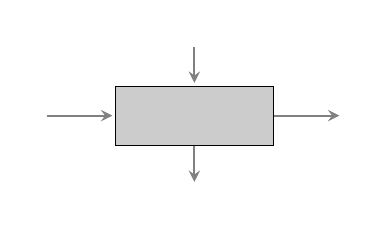
\begin{tikzpicture}[shorten >=1pt, ->, draw=black!50, node distance=1cm]
      \tikzstyle{arrow} = [thick, ->, >=stealth]
      \tikzstyle{startstop} = [rectangle, minimum width=2cm, minimum height=.75cm, text centered, draw=black, fill=black!20]
      \node (input) [] at (0cm, 1cm) {};
      \node (output) [] at (0cm, -1cm) {};
      \node (s-input) [] at (-2cm, 0cm) {};
      \node (s-output) [] at (2cm, 0cm) {};
      \path[] node[startstop] (N) at (0cm, 0cm) {};
      \draw [arrow] (input) -- (N);
      \draw [arrow] (s-input) -- (N);
      \draw [arrow] (N) -- (output);
      \draw [arrow] (N) -- (s-output);
  \end{tikzpicture}
  \end{center}
\end{frame}

\begin{frame}{Recurrent Neural Networks}
  \begin{itemize}
  \item Just like any regular neural network layer, recurrent nodes can be composed.
  \item The composition of two recurrent nodes is done by feeding the output of one node into the input of the other, and concatenating their state space.
  \item Formally, if $f:\R^n\times \R^\ell\times\R^m\to \R^k\times \R^\ell$ and $g:\R^k\times \R^\ell\times\R^m\to \R^q\times \R^\ell$ are two recurrent nodes, $$(f;g):\R^m\times\R^\ell\times\R^m\to\R^q\times\R^\ell\times\R^l$$ defined by $$(f;g)(\x, \s_1, \s_2) = (\y, \s'_1, \s'_2)$$ where $$f(\x, \s_1) = \x', \s'_1$$ and $$g(\x', \s_2) = \y, \s'_2$$.
\end{itemize}
\end{frame}

\begin{frame}{Recurrent Neural Networks}
  Graphically, we can represent this by stacking the boxes representing $f$ and $g$ on top of one another:

  \begin{center}
  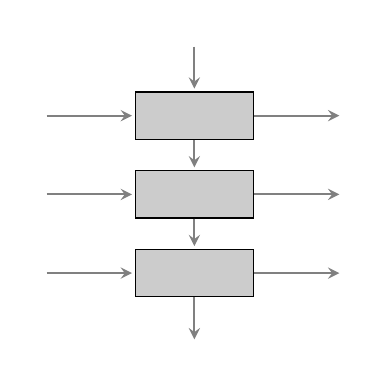
\begin{tikzpicture}[shorten >=1pt, ->, draw=black!50, node distance=1cm]
      \tikzstyle{arrow} = [thick, ->, >=stealth]
      \tikzstyle{startstop} = [rectangle, minimum width=1.5cm, minimum height=.6cm, text centered, draw=black, fill=black!20]
      \node (input) [] at (0cm, 1cm) {};
      \node (output) [] at (0cm, -3cm) {};
      \node (s-input-A) [] at (-2cm, 0cm) {};
      \node (s-output-A) [] at (2cm, 0cm) {};
      \node (s-input-B) [] at (-2cm, -1cm) {};
      \node (s-output-B) [] at (2cm, -1cm) {};
      \node (s-input-C) [] at (-2cm, -2cm) {};
      \node (s-output-C) [] at (2cm, -2cm) {};
      \path[] node[startstop] (A) at (0cm, 0cm) {};
      \path[] node[startstop] (B) at (0cm, -1cm) {};
      \path[] node[startstop] (C) at (0cm, -2cm) {};
      \draw [arrow] (input) -- (A);
      \draw [arrow] (s-input-A) -- (A);
      \draw [arrow] (s-input-B) -- (B);
      \draw [arrow] (s-input-C) -- (C);
      \draw [arrow] (A) -- (s-output-A);
      \draw [arrow] (B) -- (s-output-B);
      \draw [arrow] (C) -- (s-output-C);
      \draw [arrow] (A) -- (B);
      \draw [arrow] (B) -- (C);
      \draw [arrow] (C) -- (output);
  \end{tikzpicture}
  \end{center}
\end{frame}

\begin{frame}{Training RNN's}
  How do we train recurrent neural networks? We use a variant of back propagation, just like a regular neural network. Heuristically, we unroll the recurrent network ``infinitely'' many times, until it looks like an ordinary very deep neural network.  In practice, we only unroll the network a large but finite number of times, and treat it like an ordinary neural network.

  \begin{tikzpicture}[shorten >=1pt, ->, draw=black!50, node distance=1cm]
      \tikzstyle{arrow} = [thick, ->, >=stealth]
      \tikzstyle{startstop} = [rectangle, minimum width=1.5cm, minimum height=.6cm, text centered, draw=black, fill=black!20]
      \node (input) [] at (0cm, 1cm) {};
      \node (output) [] at (0cm, -1cm) {};
      \node (s-input-A) [] at (-2cm, 0cm) {};
      \node (s-output-A) [] at (9.5cm, 0cm) {};
      %\node (s-input-B) [] at (-2cm, -1cm) {};
      %\node (s-output-B) [] at (10cm, -1cm) {};
      %\node (s-input-C) [] at (-2cm, -2cm) {};
      %\node (s-output-C) [] at (10cm, -2cm) {};
      \path[] node[startstop] (A-0) at (0cm, 0cm) {};
      %\path[] node[startstop] (B-0) at (0cm, -1cm) {};
      %\path[] node[startstop] (C-0) at (0cm, -2cm) {};
      \draw [arrow] (input) -- (A);
      \draw [arrow] (s-input-A) -- (A-0);
      %\draw [arrow] (s-input-B) -- (B-0);
      %\draw [arrow] (s-input-C) -- (C-0);
      %\draw [arrow] (A) -- (B);
      %\draw [arrow] (B) -- (C);
      \draw [arrow] (A) -- (output);

       \foreach \i/\j in {1/0, 2/1, 3/2, 4/3}
       {
         \node (input-\i) [] at (2*\i cm, 1cm) {};
         \node (output-\i) [] at (2*\i cm, -1cm) {};
         \path[] node[startstop] (A-\i) at (2*\i cm, 0cm) {};
      %   \path[] node[startstop] (B-\i) at (2*\i cm, -1cm) {};
    %     \path[] node[startstop] (C-\i) at (2*\i cm, -2cm) {};
    %     \draw [arrow] (A-\i) -- (B-\i);
  %       \draw [arrow] (B-\i) -- (C-\i);
         \draw [arrow] (input-\i) -- (A-\i);
         \draw [arrow] (A-\j) -- (A-\i);
  %       \draw [arrow] (B-\j) -- (B-\i);
  %       \draw [arrow] (C-\j) -- (C-\i);
         \draw [arrow] (A-\i) -- (output-\i);
       }
       \draw [arrow] (A-4) -- (s-output-A);
       %\draw [arrow] (B-4) -- (s-output-B);
       %\draw [arrow] (C-4) -- (s-output-C);

  \end{tikzpicture}

\end{frame}


\begin{frame}{The Basic RNN Cell}
  We begin with the most basic of recurrent cell.
  \begin{itemize}
    \item Abstractly, a function $f:U\times S\to V\times S$ can be defined using two functions $u:\R^n\times \R^\ell\to \R^n$ and $v:\R^n\times\R^\ell \to \R^\ell$.
    \item The former function as providing the output
    \item The latter function as a state updating function.
    \item The most common definition for $u$ and $v$ for basic recurrent cells is as follows: $u(x, s) = f(A_ux+B_us)$, and $v(x, s) = \tanh(A_vx+B_vs)$, where
    \begin{itemize}
      \item $A_u$, $A_v$, $B_u$ and $B_v$ are matrices,
      \item $f$ is a non-linear function
    \end{itemize}
  \end{itemize}
\end{frame}

\defverbatim[colored]\lstI{
\begin{lstlisting}[language=Python, basicstyle=\ttfamily, keywordstyle=\color{red}]
def basic_rnn_cell(i_tensor, s_tensor, o_dim):
  i_dim = input_tensor.get_shape()[1]
  s_dim = input_tensor.get_shape()[1]
  A_u = tf.Variable(shape=[i_dim, o_dim])
  B_u = tf.Variable(shape=[s_dim, o_dim])
  A_v = tf.Variable(shape=[i_dim, s_dim])
  B_v = tf.Variable(shape=[s_dim, s_dim])
  o_tensor = tf.relu(tf.matmul(i_tensor, A_u) + \
                     tf.matmul(s_tensor, B_u))
  ns_tensor = tf.tanh(tf.matmul(i_tensor, A_v) + \
                      tf.matmul(s_tensor, B_v))
  return o_tensor, ns_tensor
\end{lstlisting}
}
\begin{frame}{The Basic RNN Cell (code)}
  In tensorflow, the code looks like:

\lstI
\end{frame}


\begin{frame}{The Long-Short-Term-Memory Cell}

\begin{itemize}
  \item It is a cell that can remember elements of a sequence it has already seen
  \item Its state has two parts: a state and a memory vector;
  \item A special {\em forget gate} controls how much of the memory vector gets forgotten
  \item An {\em input gate} controls how new information gets stored into the memory vector
  \item The usual state update and output functions
\end{itemize}
\end{frame}


\begin{frame}{The Long-Short-Term-Memory Cell}
We define:
  %There are a few problems with the architecture described above.  First, it suffers greatly from the vanishing gradient problem, since there is no way to prevent gradients from becoming very small.  Secondly, simple recurrent networks have a hard time remembering facts about the input sequence.  To remedy this situation, long short-term memory cells were introduced.
  %The overall structure of an LSTM cell is almost the same as the basic RNN cell: $f:\R^n\times \times \R^{\ell}\to \R^m\times \R^{\ell}$ which can be divided as two function
  \begin{itemize}
  \item $u:\R^{n}\times\R^m\times \R^{\ell}\to \R^m$ and
  \item $v:\R^n\times \R^m\times\R^{\ell}\to \R^{\ell}$
  \end{itemize}

  using auxiliary functions $F$, $I$, $O$, and $S$ defined as follows
  \begin{eqnarray*}
    F(x, y) &=& \sigma(A_Fx + B_Fy + b_F)\\
    I(x, y) &=& \sigma(A_Ix + B_Iy + b_I)\\
    O(x, y) &=& \sigma(A_Ox + B_Oy + b_O)\\
    S(x, y) &=& \tanh(A_Ox + B_Oy + b_O)\\
  \end{eqnarray*}
%\end{frame}
%
%
%
%\begin{frame}{The LSTM Cell}
  The state update is given by $$v(x, y, s) = F(x, y)\circ s + I(x, y)\circ \sigma_v(A_vx + B_vy + b_v)$$ where $\circ$ denotes pointwise multiplication of vectors, and finally, the output can be defined as $$u(x, y, s)=O(x, y)\circ \sigma_u(v(x, y, s))$$\

\end{frame}

\defverbatim[colored]\lstI{
\begin{lstlisting}[language=Python, basicstyle=\ttfamily, keywordstyle=\color{red}]
def lstm_gate(input_tensor, previous_output, op):
  _, N = input_tensor.get_shape()
  _, output_dim = previous_output.get_shape()
  A = tf.Variable(shape=[N, output_dim])
  B = tf.Variable(shape=[output_dim, output_dim])
  b = tf.Variable(shape=[1, output_dim])
  x = tf.matmul(input_tensor, A) + \
        tf.matmul(previous_output, B) + b
  return op(x)

def lstm_cell(input_tensor, output):
  _, output_dim = output.get_shape()
  F = lstm_gate(input_tensor, output, tf.sigmoid)
  I = lstm_gate(input_tensor, output, tf.sigmoid)
  O = lstm_gate(input_tensor, output, tf.sigmoid)
  S = lstm_gate(input_tensor, output, tf.tanh)
  new_state = tf.mul(output, F) + tf.mul(I, S)
  output = tf.mul(O, tf.tanh(new_state))
  return output, new_state
\end{lstlisting}
}
\begin{frame}{The LSTM Cell (code)}
\lstI
\end{frame}


\begin{frame}{The Basic GRU Cell}
  %A common variant of the long short term memory cell is the {\em gated recurrent unit cell}, more commonly known as GRU cells.  The philosophy behind their design is similar to the long short term memory. Once again, each step of the computation takes into account a state vector and the output of the previous iteration.
  \begin{itemize}
    \item GRU's are a simplification of the LSTM cell.
    \item Compared to LSTM the GRU lacks an output gate.
    \item Its performance is on par with LSTM cells in most applications.
  \end{itemize}
  %$f:\R^n\times \R^m\times \R^{\ell}\to \R^m\times \R^{\ell}$, which can be divided as two function
  %\begin{itemize}
  %  $u:\R^{n}\times\R^m\times \R^{\ell}\to \R^m$
  %   $v:\R^n\times \R^m\times\R^{\ell}\to \R^{\ell}$
  %   \end{itemize}
  To define the functions $u$ and $v$, we use auxiliary functions $U$(pdate) and  $R$(eset) defined as follows
  \begin{eqnarray*}
    U(x, y) &=& \sigma(A_Ux + B_Uy + b_U)\\
    R(x, y) &=& \sigma(A_Rx + B_Ry + b_R)\\
  \end{eqnarray*}
  The state update (and output) is given by $$v(x, y, s) = U(x, y)\circ s + (1-s)\circ \sigma_h(A_v x + B_v(R(x, y)\circ y) + b_v)$$
  %The output is the same as the state.
\end{frame}


\defverbatim[colored]\lstI{
\begin{lstlisting}[language=Python, basicstyle=\ttfamily, keywordstyle=\color{red}]
def gru_gate(input_tensor, previous_output, port_op):
  _, N = input_tensor.get_shape()
  _, output_dim = previous_output.get_shape()
  A = tf.Variable(shape=[N, output_dim])
  B = tf.Variable(shape=[output_dim, output_dim])
  b = tf.Variable(shape=[output_dim, output_dim])
  x = tf.matmul(input_tensor, A) + \
        tf.matmul(previous_output, B) + b
  return post_op(x)

def gru_cell(input_tensor, output, state):
  U = gru_gate(input_tensor, output, tf.sigmoid)
  R = gru_gate(input_tensor, output, tf.sigmoid)
  O = gru_gate(input, tf.mul(R, output))
  return [tf.mul(R, output) + tf.mul((1-R), O)]*2
\end{lstlisting}
}
\begin{frame}{The GRU Cell (code)}
\lstI
\end{frame}






\begin{frame}{A many-to-one example}
\begin{itemize}
  \item As an example of a many-to-one RNN, consider the Buzzometer sentiment analysis tool.
  \item On input of a sequence of {\bf characters}, we output one of 4 classes: negative, neutral, positive and irrelevant.
  \item For training, the network was unrolled to 256 characters, which is twise the average length of a message in out database.
  \item Longer messaages were truncated, and shorter messages were padded with $0$.
\end{itemize}

The architecture is:
\begin{itemize}
  \item A 3 layer {\em bi-directional RNN}
  \item We keep the last output of the forward and the backward networks, and combine them linearly: $\w=W_1 \v_f + W_2\v_b$
  \item The vector $\w$ is then projected to $\R^4$.
\end{itemize}
\end{frame}

\begin{frame}{A many-to-one example (model architecture)}
  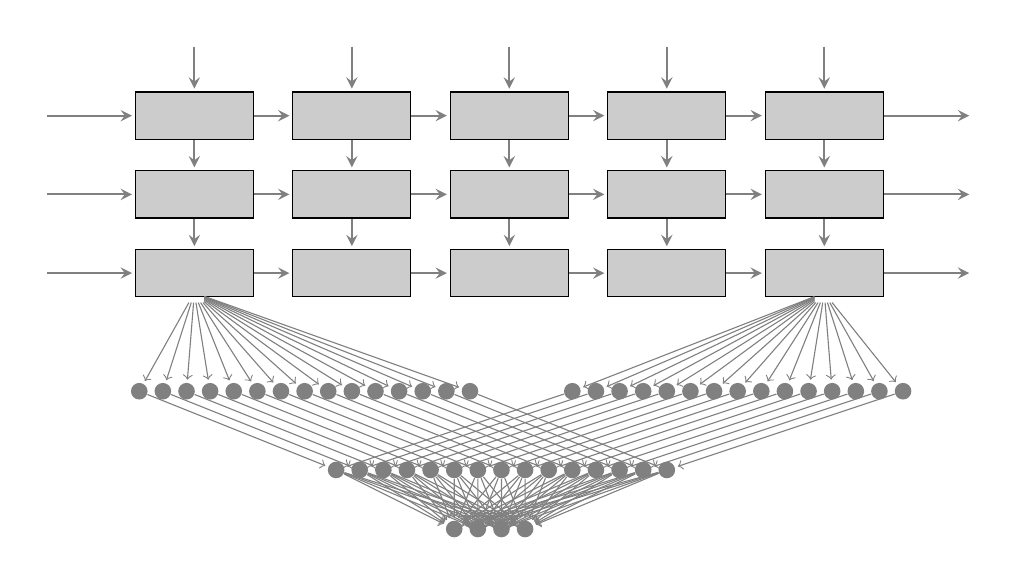
\begin{tikzpicture}[shorten >=1pt, ->, draw=black!50, node distance=1cm]
      \tikzstyle{arrow} = [thick, ->, >=stealth]
       \tikzstyle{every pin edge}=[<-, shorten <=1pt]
       \tikzstyle{neuron}=[circle, fill=black!50, minimum size=6pt, inner sep=0pt]

      \tikzstyle{startstop} = [rectangle, minimum width=1.5cm, minimum height=.6cm, text centered, draw=black, fill=black!20]
      \node (input) [] at (0cm, 1cm) {};
      \node (output) [] at (0cm, -2.25cm) {};
      \node (s-input-A) [] at (-2cm, 0cm) {};
      \node (s-output-A) [] at (10cm, 0cm) {};
      \node (s-input-B) [] at (-2cm, -1cm) {};
      \node (s-output-B) [] at (10cm, -1cm) {};
      \node (s-input-C) [] at (-2cm, -2cm) {};
      \node (s-output-C) [] at (10cm, -2cm) {};
      \path[] node[startstop] (A-0) at (0cm, 0cm) {};
      \path[] node[startstop] (B-0) at (0cm, -1cm) {};
      \path[] node[startstop] (C-0) at (0cm, -2cm) {};
      \draw [arrow] (input) -- (A-0);
      \draw [arrow] (s-input-A) -- (A-0);
      \draw [arrow] (s-input-B) -- (B-0);
      \draw [arrow] (s-input-C) -- (C-0);
      \draw [arrow] (A-0) -- (B-0);
      \draw [arrow] (B-0) -- (C-0);
      %\draw [arrow] (C) -- (output);

       \foreach \i/\j in {1/0, 2/1, 3/2, 4/3}
       {
         \node (input-\i) [] at (2*\i cm, 1cm) {};
         \node (output-\i) [] at (2*\i cm, -2.25cm) {};
         \path[] node[startstop] (A-\i) at (2*\i cm, 0cm) {};
         \path[] node[startstop] (B-\i) at (2*\i cm, -1cm) {};
         \path[] node[startstop] (C-\i) at (2*\i cm, -2cm) {};
         \draw [arrow] (A-\i) -- (B-\i);
         \draw [arrow] (B-\i) -- (C-\i);
         \draw [arrow] (input-\i) -- (A-\i);
         \draw [arrow] (A-\j) -- (A-\i);
         \draw [arrow] (B-\j) -- (B-\i);
         \draw [arrow] (C-\j) -- (C-\i);
         %5\draw [arrow] (C-\i) -- (output-\i);
       }
       \draw [arrow] (A-4) -- (s-output-A);
       \draw [arrow] (B-4) -- (s-output-B);
       \draw [arrow] (C-4) -- (s-output-C);

       \foreach \name / \x in {1, ..., 15} {
           \path[xshift=-1cm]
               node[neuron] (I-\name) at (0.3*\x, -3.5cm) {};
               \path (output) edge (I-\name);
               }

       \foreach \name / \x in {1, ..., 15} {
           \path[xshift=4.5cm]
               node[neuron] (J-\name) at (0.3*\x, -3.5cm) {};
              \path (output-4) edge (J-\name); }

       \foreach \name / \x in {1, ..., 15}{
           \path[xshift=1.5cm]
               node[neuron] (K-\name) at (0.3*\x, -4.5cm) {};
          \path (I-\name) edge (K-\name);
          \path (J-\name) edge (K-\name); }

          \foreach \name / \x in {1, ..., 4}{
              \path[xshift=3cm] node[neuron] (O-\name) at (0.3*\x, -5.25cm) {};
              \foreach \j in {1, ..., 15}{
             \path (K-\j) edge (O-\name);}
             }
  \end{tikzpicture}

\end{frame}


\defverbatim[colored]\lstI{
\begin{lstlisting}[language=Python, basicstyle=\ttfamily, keywordstyle=\color{red}]
model_input = tf.placeholder(shape=[SEQ_LENGTH])
_ = tf.one_hot(model_input, depth=E_DIM, axis=-1)
_ = tf.reshape(_, [-1, SEQ_LENGTH, E_DIM])
fw = multi_layer_rnn(N_LAYERS, STATE_DIM)
bw = multi_layer_rnn(N_LAYERS, STATE_DIM)
OP = tf.nn.bidirectional_dynamic_rnn
output, _ = OP(fw, bw, _, dtype=tf.float32)
fw_output = tf.reshape(output[0][:, -1:],
                            [-1, STATE_DIM])
bw_output = tf.reshape(output[1][:, :1],
                            [-1, STATE_DIM])
f = project(fw_output, E_DIM)
b = project(bw_output, E_DIM)
e = tf.add(f, b)
model_output = project(e, NUM_CLASSES)
prediction = tf.argmax(model_output, 1)
\end{lstlisting}
}
\begin{frame}{A many-to-one example (code)}
\lstI
\end{frame}

\begin{frame}{A many-to-one example (output)}
\begin{center}
  \begin{tabular}{lcccc}
    {} & {\bf Negative} & {\bf Neutral} & {\bf Positive} & {\bf Irrelevant}\\
    {\bf Negative}   & {291} & {113} & {50} & {127}\\
    {\bf Neutral}    & {108} & {113} & {50} & {85}\\
    {\bf Positive}   & {0} & {0} & {0} & {0}\\
    {\bf Irrelevant} & {0} & {0} & {0} & {0}\\
  \end{tabular}
\end{center}
%\end{frame}
%
%\begin{frame}{A many-to-one example (output)}
  \begin{center}
  \begin{tabular}{lcccc}
    {} & {\bf Negative} & {\bf Neutral} & {\bf Positive} & {\bf Irrelevant}\\
    {\bf Negative}   & {292} & {52} & {36} & {55}\\
    {\bf Neutral}    & {61} & {176} & {21} & {62}\\
    {\bf Positive}   & {5} & {15} & {65} & {15}\\
    {\bf Irrelevant} & {33} & {28} & {14} & {70}\\
  \end{tabular}
\end{center}

%\end{frame}
%
%\begin{frame}{A many-to-one example (output)}
  \begin{center}
  \begin{tabular}{lcccc}
    {} & {\bf Negative} & {\bf Neutral} & {\bf Positive} & {\bf Irrelevant}\\
    {\bf Negative}   & {319} & {38} & {11} & {43}\\
    {\bf Neutral}    & {20} & {188} & {2} & {20}\\
    {\bf Positive}   & {10} & {18} & {91} & {10}\\
    {\bf Irrelevant} & {27} & {27} & {7} & {169}\\
  \end{tabular}
\end{center}
\end{frame}

\begin{frame}{A many-to-one example (output)}
  \begin{center}
  \begin{tabular}{lcccc}
    {} & {\bf Negative} & {\bf Neutral} & {\bf Positive} & {\bf Irrelevant}\\
    {\bf Negative}   & {334} & {4} & {4} & {9}\\
    {\bf Neutral}    & {3} & {283} & {2} & {7}\\
    {\bf Positive}   & {1} & {0} & {125} & {2}\\
    {\bf Irrelevant} & {1} & {0} & {4} & {221}\\
  \end{tabular}
\end{center}
%
%\end{frame}
%
%\begin{frame}{A many-to-one example (output)}
  \begin{center}
  \begin{tabular}{lcccc}
    {} & {\bf Negative} & {\bf Neutral} & {\bf Positive} & {\bf Irrelevant}\\
    {\bf Negative}   & {321} & {16} & {3} & {20}\\
    {\bf Neutral}    & {8} & {286} & {4} & {6}\\
    {\bf Positive}   & {4} & {2} & {125} & {16}\\
    {\bf Irrelevant} & {11} & {9} & {1} & {168}\\
  \end{tabular}
\end{center}
\end{frame}



\begin{frame}{A many-to-many example}
  \begin{itemize}
    \item we define an architecture that generates text in the style of a particular author, or body of text.
    \item The architecture is very simple, and consists of three stacked GRU cells.
    \item This model will also expose some of the challenges in training recurrent networks.
  \end{itemize}
\end{frame}

\begin{frame}{A many-to-many example (model architecture)}
  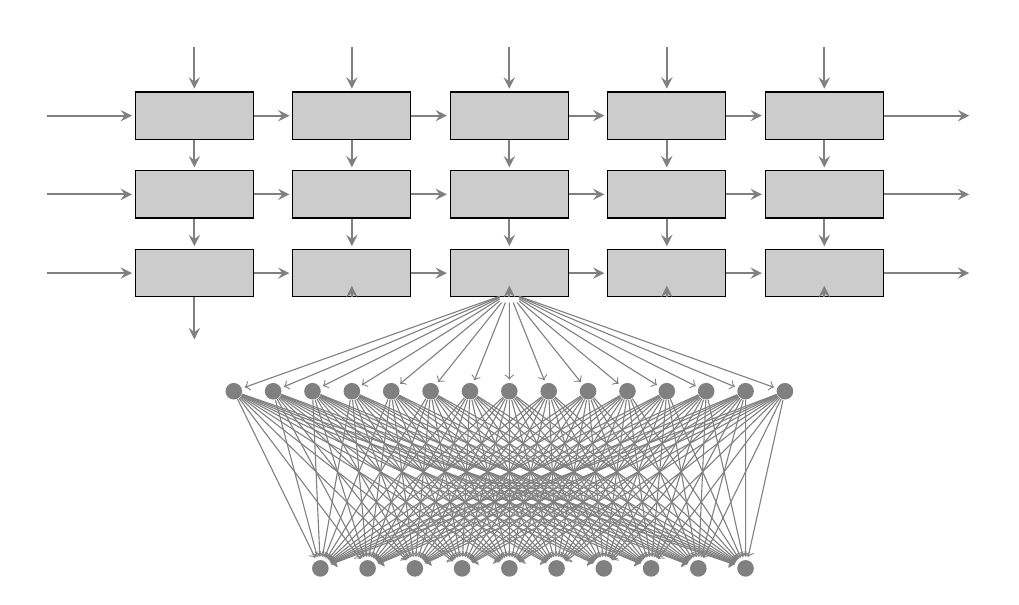
\begin{tikzpicture}[shorten >=1pt, ->, draw=black!50, node distance=1cm]
      \tikzstyle{arrow} = [thick, ->, >=stealth]
      \tikzstyle{startstop} = [rectangle, minimum width=1.5cm, minimum height=.6cm, text centered, draw=black, fill=black!20]
      \tikzstyle{neuron}=[circle, fill=black!50, minimum size=6pt, inner sep=0pt]

      \node (input) [] at (0cm, 1cm) {};
      \node (output) [] at (0cm, -3cm) {};
      \node (s-input-A) [] at (-2cm, 0cm) {};
      \node (s-output-A) [] at (10cm, 0cm) {};
      \node (s-input-B) [] at (-2cm, -1cm) {};
      \node (s-output-B) [] at (10cm, -1cm) {};
      \node (s-input-C) [] at (-2cm, -2cm) {};
      \node (s-output-C) [] at (10cm, -2cm) {};
      \path[] node[startstop] (A-0) at (0cm, 0cm) {};
      \path[] node[startstop] (B-0) at (0cm, -1cm) {};
      \path[] node[startstop] (C-0) at (0cm, -2cm) {};
      \draw [arrow] (input) -- (A-0);
      \draw [arrow] (s-input-A) -- (A-0);
      \draw [arrow] (s-input-B) -- (B-0);
      \draw [arrow] (s-input-C) -- (C-0);
      \draw [arrow] (A-0) -- (B-0);
      \draw [arrow] (B-0) -- (C-0);
      \draw [arrow] (C-0) -- (output);

       \foreach \i/\j in {1/0, 2/1, 3/2, 4/3}
       {
         \node (input-\i) [] at (2*\i cm, 1cm) {};
         \node (output-\i) [] at (2*\i cm, -2.25cm) {};
         \path[] node[startstop] (A-\i) at (2*\i cm, 0cm) {};
         \path[] node[startstop] (B-\i) at (2*\i cm, -1cm) {};
         \path[] node[startstop] (C-\i) at (2*\i cm, -2cm) {};
         \draw [arrow] (A-\i) -- (B-\i);
         \draw [arrow] (B-\i) -- (C-\i);
         \draw [arrow] (input-\i) -- (A-\i);
         \draw [arrow] (A-\j) -- (A-\i);
         \draw [arrow] (B-\j) -- (B-\i);
         \draw [arrow] (C-\j) -- (C-\i);
         \draw [arrow] (C-\i) -- (output-\i);
       }
       \draw [arrow] (A-4) -- (s-output-A);
       \draw [arrow] (B-4) -- (s-output-B);
       \draw [arrow] (C-4) -- (s-output-C);

       \foreach \name / \x in {1, ..., 15}{
           \path[xshift=0cm]
               node[neuron] (K-\name) at (0.5*\x, -3.5cm) {};
          \path (output-2) edge (K-\name);
          %\path (J-\name) edge (K-\name);
          }

          \foreach \name / \x in {1, ..., 10}{
              \path[xshift=1cm] node[neuron] (O-\name) at (0.6*\x, -5.75cm) {};
              \foreach \j in {1, ..., 15}{
             \path (K-\j) edge (O-\name);}
             %\path (J-\name) edge (K-\name);
             }
  \end{tikzpicture}
\end{frame}

\begin{frame}{A many-to-one example (output)}
\begin{itemize}
  \item For training we network was unrolled to 30 characters, and the training was done in batches of 32 strings.
  \item The main challenge for training is that the strings should continue from batch to batch.  \item For example, consider training a similar network unrolled to 2 characters with a batch size of 3.
  \item Consider the sentence {\tt The quick brown fox jumps over the lazy dog}.
  \item The first step is to cut the string into substrings of length 2:
  {\tt |Th|e\textvisiblespace |qu|ic|k\textvisiblespace |br|ow|n\textvisiblespace |fo|x\textvisiblespace |ju|mp|s\textvisiblespace |ov|er| \textvisiblespace t|he|\textvisiblespace l|az|y\textvisiblespace |do|g.|}.
  \item In a normal batching situation, we would then cut this liet of strings into chunks of length 3, like so:
{\tt |(Th|e\textvisiblespace |qu)|(ic|k\textvisiblespace |br)|(ow|n\textvisiblespace |fo)|(x\textvisiblespace |ju|mp)| (s\textvisiblespace |ov|er)|(\textvisiblespace t|he|\textvisiblespace l)|(az|y\textvisiblespace |do)|} but this causes a problem.
\end{itemize}
\end{frame}

\begin{frame}{A many-to-many example (output)}

    {\tt |Th|e\textvisiblespace |qu|ic|k\textvisiblespace |br|ow|n\textvisiblespace |fo|x\textvisiblespace |ju|mp|s\textvisiblespace |ov|er|\textvisiblespace t|he|\textvisiblespace l|az|y |do|g.|}.

    {\tt |(Th|e\textvisiblespace |qu)|(ic|k\textvisiblespace |br)|(ow|n\textvisiblespace |fo)|(x |ju|mp)|(s\textvisiblespace |ov|er)|(\textvisiblespace t|he|\textvisiblespace l)|(az|y\textvisiblespace |do)|}

  \begin{itemize}
\item The first sequence of the first batch is {\tt Th}, which will leave the network in a certain state $s$. \item For this state to be updated properly, the first element of the second batch should be {\tt |e\textvisiblespace |}, and {\em not} {\tt |ic|}.
\item We must therefore use a different batching strategy. The string will give us 7 batches in total, so we number the subsequences with a batch index from 1 to 7 in order, starting over at 1 when we run out of indices.
\end{itemize}
\end{frame}

\begin{frame}{A many-to-one example (output)}
  \begin{center}
\begin{tabular}{ccccccc}
  {1}&{2}&{3}&{4}&{5}&{6}&{7}\\\hline
  Th & e\textvisiblespace &  qu & ic & k\textvisiblespace &  br & ow \\
  n\textvisiblespace & fo & x\textvisiblespace &  ju & mp & s\textvisiblespace &  ov \\
   er & \textvisiblespace t & he & \textvisiblespace l & az & y\textvisiblespace &  do \\
  g. &  {}&{}&{}&{}&{}&{}
\end{tabular}
\end{center}
\end{frame}

\defverbatim[colored]\lstI{
\begin{lstlisting}[language=Python, basicstyle=\ttfamily, keywordstyle=\color{red}]
model_input = tf.placeholder(shape=[None, SEQ_LENGTH])
initial_state = tf.placeholder(shape=[N_LAYERS, S_DIM])
_ = tf.one_hot(model_input, depth=E_DIM, axis=-1)
encode = multi_layer_rnn(N_LAYERS, STATE_DIM)
state_tuple = tuple(tf.unstack(initial_state, axis=0))
OP = tf.nn.dynamic_rnn
output, state = OP(encode, _,
                   dtype=tf.float32,
                   initial_state=state_tuple)
output = tf.reshape(output, [-1, STATE_DIM])
output = project(output, E_DIM)
out = tf.reshape(out, [-1, SEQ_LENGTH])
model_output = tf.nn.softmax(output)
output = tf.argmax(output, 1)
\end{lstlisting}
}

\begin{frame}{A many-to-many example (code)}
\lstI
\end{frame}



\defverbatim[colored]\lstI{
\begin{lstlisting}[language=Python, basicstyle=\ttfamily, keywordstyle=\color{red}]
def generate_text(length, session=None):
    generated_text = ''
    character = [[ord(' ')]]
    istate = np.zeros([N_LAYERS, 1, STATE_DIM])
    while len(generated_text) < length:
        feed_dict = {model_input: character,
                     initial_state: istate}
        next_char, state = session.run(
          [out, state], feed_dict=feed_dict)
        op = np.random.multinomial
        next_char_id = op(1, next_char.squeeze(), 1)
        next_char_id = next_char_id.argmax()
        next_char_id = next_char_id \
                if chr(next_char_id) in \
                    string.printable else ord(" ")
        generated_text += chr(next_char_id)
        character = [[next_char_id]]
        istate = state
    return generated_text
\end{lstlisting}
}


\begin{frame}{A many-to-many example (text generating)}
\lstI
\end{frame}



\begin{frame}{A many-to-many example (output)}

\end{frame}

\begin{frame}{A many-to-many example (output)}

\end{frame}

\begin{frame}{A many-to-many example (output)}

\end{frame}

\begin{frame}{A many-to-many example (output)}

\end{frame}

\begin{frame}{A many-to-many example (output)}

\end{frame}

\begin{frame}{A many-to-many example (output)}

\end{frame}

\begin{frame}{A many-to-many example (output)}

\end{frame}

\begin{frame}{A many-to-many example (output)}

\end{frame}

\begin{frame}{A many-to-many example (output)}

\end{frame}

\begin{frame}{A many-to-many example (output)}

\end{frame}

\begin{frame}{A many-to-many example (output)}

\end{frame}

\begin{frame}{A many-to-many example (output)}

\end{frame}



\begin{frame}{Many-to-one-to-many example}


\begin{itemize}
\item  A recurrent neural network that can sort sequences
\item Two parts: an encoder, and a decoder
\item The encoder encodes sequences into fixed length vectors
\item The decoder transforms this vector into a sorted list of numbers.
\item For simplicity, the model was restricted to sequences of length 32
\item the elements of the sequence were all betweeen 1 and 128
\end{itemize}

 \end{frame}



 \begin{frame}{Many-to-one-to-many example}

   \begin{tikzpicture}[shorten >=1pt, ->, draw=black!50, node distance=1cm]
       \tikzstyle{arrow} = [thick, ->, >=stealth]
       \tikzstyle{startstop} = [rectangle, minimum width=1.5cm, minimum height=.6cm, text centered, draw=black, fill=black!20]
       \node (input) [] at (0cm, 1cm) {};
       \node (output) [] at (0cm, -1cm) {};
       \node (s-input-A) [] at (-2cm, 0cm) {};
       \node (s-output-A) [] at (7.5cm, 0cm) {};
       \path[] node[startstop] (A-0) at (0cm, 0cm) {};
       \draw [arrow] (input) -- (A);
       \draw [arrow] (s-input-A) -- (A-0);
       \draw [arrow] (A) -- (output);

        \foreach \i/\j in {1/0, 2/1, 3/2}
        {
          \node (input-\i) [] at (2*\i cm, 1cm) {};
          \node (output-\i) [] at (2*\i cm, -1cm) {};
          \path[] node[startstop] (A-\i) at (2*\i cm, 0cm) {};
          \draw [arrow] (input-\i) -- (A-\i);
          \draw [arrow] (A-\j) -- (A-\i);
          \draw [arrow] (A-\i) -- (output-\i);
        }

        \draw [arrow] (A-3) -- (s-output-A);

        \node (d-input) [] at (0cm, -2cm) {};
        \node (d-output) [] at (0cm, -4cm) {};
        \node (d-s-input-A) [] at (-2cm, -3cm) {};
        \node (d-s-output-A) [] at (7.5cm, -3cm) {};
        \path[] node[startstop] (d-A-0) at (0cm, -3cm) {};
        \draw [arrow] (d-input) -- (d-A-0);
        \draw [arrow] (d-s-input-A) -- (d-A-0);
        \draw [arrow] (d-A-0) -- (d-output);

         \foreach \i/\j in {1/0, 2/1, 3/2}
         {
           \node (d-input-\i) [] at (2*\i cm, -2cm) {};
           \node (d-output-\i) [] at (2*\i cm, -4cm) {};
           \path[] node[startstop] (d-A-\i) at (2*\i cm, -3cm) {};
           \draw [arrow] (d-input-\i) -- (d-A-\i);
           \draw [arrow] (d-A-\j) -- (d-A-\i);
           \draw [arrow] (d-A-\i) -- (d-output-\i);
         }
         \draw [arrow] (d-A-3) -- (d-s-output-A);

         \draw [arrow] (output-3) -- (d-input);

   \end{tikzpicture}
 \end{frame}


 \defverbatim[colored]\lstI{
 \begin{lstlisting}[language=Python, basicstyle=\ttfamily, keywordstyle=\color{red}]
model_input = tf.placeholder('uint8',
                      shape=[None, SEQ_LENGTH])
_ = tf.one_hot(model_input, depth=E_DIM, axis=-1)
_ = tf.reshape(_, [-1, SEQ_LENGTH, E_DIM])
encode = multi_layer_rnn(N_LAYERS, STATE_DIM)
OP = tf.nn.dynamic_rnn
encoded_input, state = OP(encode, _, dtype=tf.float32)
encoder_output = state
 \end{lstlisting}
 }
 \begin{frame}{Many-to-one-to-many example (code for encoder)}
   \lstI
 \end{frame}


 \defverbatim[colored]\lstI{
 \begin{lstlisting}[language=Python, basicstyle=\ttfamily, keywordstyle=\color{red}]
with tf.variable_scope('decoder'):
   training_decoder_input = \
          tf.zeros_like(Globals.model_input)
   _ = tf.one_hot(training_decoder_input,
                  depth=E_DIM, axis=-1)
   _ = tf.reshape(_, [-1, SEQ_LENGTH, E_DIM])
   decode = multi_layer_rnn(N_LAYERS, STATE_DIM)
   OP = tf.nn.dynamic_rnn
   decoded_output, state = OP(decode, _,
                              dtype=tf.float32,
                              initial_state=state)
   decoded_output = tf.reshape(decoded_output,
                               [-1, STATE_DIM])
   output = project(decoded_output, E_DIM)
   out = tf.argmax(output, 1)
 \end{lstlisting}
 }
 \begin{frame}{Many-to-one-to-many example (code for decoder)}
   \lstI
 \end{frame}


 \begin{frame}{A many-to-one-to-many example (output)}
   \begin{itemize}
   \item 39, 9, 113, 57, 39, 124, 125, 86, 65, 30, 39, 124, 98, 65, 27, 62, 79, 102, 96, 45, 96, 42, 54, 92, 33, 61, 14, 106, 89, 4, 61, 95;
   \item 57, 6, 6, 6, 6, 6, 96, 96, 96, 96, 96, 96, 96, 96, 96, 96, 96, 118, 118, 118, 118, 118, 118, 118, 118, 118, 118, 118, 118, 118, 118, 118
  \end{itemize}
  \begin{itemize}
   \item 22, 31, 58, 43, 96, 83, 95, 65, 17, 48, 65, 122, 94, 109, 113, 49, 74, 61, 39, 127, 3, 14, 107, 91, 55, 2, 108, 7, 119, 60, 32, 21;
   \item 14, 14, 14, 17, 17, 6, 6, 6, 96, 96, 96, 96, 96, 96, 96, 118, 118, 118, 118, 118, 118, 118, 118, 118, 118, 118, 118, 118, 118, 118, 118, 118
 \end{itemize}
 \begin{itemize}
   \item 117, 15, 77, 4, 57, 121, 108, 76, 72, 119, 41, 4, 94, 44, 103, 124, 120, 20, 79, 121, 68, 12, 31, 97, 93, 19, 45, 27, 119, 92, 119, 92;
   \item 65, 65, 95, 95, 95, 96, 96, 96, 96, 96, 96, 96, 96, 96, 96, 96, 96, 118, 118, 118, 118, 118, 118, 118, 118, 118, 118, 118, 118, 118, 118, 118
 \end{itemize}
 \end{frame}

 \begin{frame}{A many-to-one-to-many example (output)}
 \begin{itemize}
   \item 75, 6, 57, 57, 108, 34, 78, 71, 112, 115, 108, 48, 67, 1, 14, 9, 14, 115, 83, 62, 86, 91, 61, 40, 105, 92, 86, 84, 30, 84, 19, 107;
   \item 1, 6, 9, 14, 14, 19, 0, 34, 40, 48, 57, 57, 61, 62, 67, 71, 75, 78, 83, 84, 84, 85, 86, 91, 92, 105, 107, 107, 109, 111, 114, 115
 \end{itemize}
 \begin{itemize}
   \item 59, 108, 56, 66, 76, 38, 100, 61, 47, 79, 102, 15, 24, 92, 8, 26, 126, 43, 5, 90, 41, 2, 60, 85, 2, 104, 86, 40, 35, 47, 61, 91;
   \item 2, 2, 5, 8, 15, 24, 26, 35, 38, 40, 41, 42, 47, 47, 56, 59, 60, 61, 61, 66, 76, 79, 84, 86, 89, 91, 92, 100, 102, 104, 108, 126
 \end{itemize}
 \begin{itemize}
   \item 25, 50, 64, 4, 40, 47, 6, 14, 97, 32, 87, 103, 44, 25, 84, 40, 95, 13, 113, 66, 38, 79, 106, 40, 26, 16, 74, 50, 119, 32, 80, 16;
   \item 4, 6, 13, 14, 16, 16, 25, 25, 26, 32, 32, 38, 39, 40, 40, 44, 47, 50, 50, 64, 66, 74, 79, 80, 84, 86, 95, 97, 103, 106, 113, 119
 \end{itemize}
 \end{frame}

 \begin{frame}{A many-to-one-to-many example (output)}
 \begin{itemize}
   \item 96, 59, 77, 29, 39, 112, 23, 79, 60, 110, 97, 69, 107, 13, 96, 124, 2, 12, 55, 16, 106, 110, 30, 118, 119, 52, 22, 37, 113, 93, 73, 58;
   \item 2, 12, 13, 16, 22, 23, 29, 0, 37, 39, 52, 55, 58, 59, 60, 69, 73, 77, 79, 93, 96, 96, 97, 106, 107, 109, 111, 111, 113, 118, 119, 124
 \end{itemize}
 \begin{itemize}
   \item 44, 117, 104, 116, 111, 115, 58, 79, 8, 9, 1, 39, 112, 43, 64, 31, 126, 12, 36, 10, 93, 87, 40, 5, 108, 92, 11, 75, 113, 104, 64, 109;
   \item 1, 5, 8, 9, 10, 11, 12, 0, 36, 39, 40, 0, 44, 58, 64, 64, 75, 79, 0, 92, 93, 104, 104, 108, 109, 111, 113, 113, 115, 116, 117, 126
 \end{itemize}
 \begin{itemize}
   \item 58, 19, 10, 52, 22, 61, 67, 96, 3, 7, 116, 96, 54, 24, 19, 45, 127, 124, 11, 114, 53, 75, 126, 84, 122, 41, 75, 1, 119, 18, 92, 51;
   \item 1, 3, 7, 10, 11, 18, 19, 19, 22, 24, 41, 45, 51, 52, 53, 54, 58, 61, 67, 75, 75, 84, 92, 96, 96, 114, 116, 119, 122, 124, 126, 127
 \end{itemize}
 \end{frame}

 \begin{frame}{A many-to-one-to-many example (output)}
 \begin{itemize}
   \item 34, 73, 95, 91, 93, 108, 43, 75, 38, 70, 66, 40, 108, 127, 25, 94, 34, 26, 89, 23, 95, 43, 2, 54, 11, 19, 105, 52, 108, 77, 93, 86;
   \item 2, 11, 19, 23, 25, 26, 34, 34, 38, 40, 0, 0, 52, 54, 66, 70, 73, 75, 77, 86, 89, 91, 93, 93, 94, 95, 95, 105, 107, 108, 108, 127
 \end{itemize}
 \begin{itemize}
   \item 95, 106, 119, 69, 40, 41, 28, 114, 12, 1, 106, 87, 117, 78, 54, 37, 110, 24, 9, 114, 107, 87, 33, 76, 5, 90, 29, 14, 96, 109, 1, 3;
   \item 1, 1, 3, 5, 9, 12, 14, 24, 28, 29, 33, 37, 40, 41, 54, 69, 76, 78, 86, 0, 90, 95, 96, 106, 106, 107, 109, 110, 114, 114, 117, 119
 \end{itemize}
 \begin{itemize}
   \item 122, 97, 90, 61, 72, 66, 60, 60, 25, 125, 84, 73, 114, 46, 112, 76, 110, 62, 58, 34, 126, 124, 102, 35, 11, 100, 47, 113, 85, 64, 22, 89;
   \item 11, 22, 25, 34, 35, 46, 47, 58, 60, 60, 61, 62, 64, 66, 72, 73, 76, 84, 85, 89, 90, 97, 100, 102, 110, 113, 113, 114, 122, 124, 125, 126
 \end{itemize}
 \end{frame}

 \begin{frame}{A many-to-one-to-many example (output)}
 \begin{itemize}
   \item 69, 41, 40, 61, 9, 120, 37, 85, 103, 47, 81, 77, 126, 72, 86, 72, 6, 72, 92, 7, 22, 100, 127, 19, 89, 72, 62, 6, 64, 26, 45, 15;
   \item 6, 6, 7, 9, 15, 19, 22, 26, 37, 40, 41, 45, 47, 61, 62, 64, 69, 72, 72, 72, 72, 77, 81, 85, 86, 89, 92, 100, 103, 120, 126, 127
 \end{itemize}
 \begin{itemize}
   \item 95, 40, 116, 120, 68, 75, 24, 114, 39, 81, 52, 37, 76, 10, 15, 105, 79, 15, 44, 89, 115, 5, 26, 11, 85, 53, 85, 114, 39, 29, 34, 16;
   \item 5, 10, 11, 15, 15, 16, 24, 26, 29, 34, 37, 39, 39, 40, 44, 52, 53, 68, 75, 76, 79, 81, 85, 85, 89, 95, 105, 114, 114, 115, 116, 120
 \end{itemize}
 \begin{itemize}
   \item 20, 61, 78, 15, 61, 8, 108, 36, 85, 96, 40, 80, 106, 24, 66, 82, 96, 43, 126, 33, 80, 116, 35, 86, 98, 81, 76, 89, 6, 103, 117, 16;
   \item 6, 8, 15, 16, 20, 24, 33, 35, 36, 40, 0, 61, 61, 66, 76, 78, 80, 80, 81, 82, 85, 86, 89, 96, 96, 98, 103, 106, 108, 116, 117, 126
 \end{itemize}
 \end{frame}
\end{document}
